% =============================================================================
% Automated Asteroid Lightcurve Inversion Pipeline
% Publication-quality research paper
% =============================================================================
\documentclass[11pt,a4paper]{article}

% --- Packages ---
\usepackage[margin=1in]{geometry}
\usepackage{amsmath,amssymb}
\usepackage{algorithm}
\usepackage{algorithmic}
\usepackage{booktabs}
\usepackage{hyperref}
\usepackage[round]{natbib}
\usepackage{pgfplots}
\pgfplotsset{compat=1.18}
\usepackage{tikz}
\usetikzlibrary{shapes.geometric, arrows.meta, positioning, calc, fit, backgrounds}
\usepackage{graphicx}
\usepackage{subcaption}
\usepackage{multirow}
\usepackage{xcolor}
\usepackage{float}
\usepackage{enumitem}
\usepackage{microtype}
\usepackage{url}

% --- Custom colors ---
\definecolor{pipeblue}{RGB}{52,101,164}
\definecolor{pipeorange}{RGB}{204,120,50}
\definecolor{pipegreen}{RGB}{78,154,6}
\definecolor{pipeteal}{RGB}{32,142,142}

% --- Hyperref setup ---
\hypersetup{
  colorlinks=true,
  linkcolor=pipeblue,
  citecolor=pipeblue,
  urlcolor=pipeteal
}

% --- Title ---
\title{\textbf{Automated Asteroid Shape Modeling from Archival Photometry:\\
A Lightcurve Inversion Pipeline Integrating Convex, Genetic,\\
and Sparse Data Approaches}}

\author{Research Lab (Automated)}

\date{February 2026}

\begin{document}

\maketitle
\thispagestyle{empty}

% ============================================================================
% ABSTRACT
% ============================================================================
\begin{abstract}
Deriving three-dimensional shape models and spin states of asteroids from
disk-integrated photometry is central to planetary science, yet the majority
of asteroids with dense lightcurve archives remain unmodeled.
We present a fully automated, open-source pipeline for asteroid lightcurve
inversion that processes the Asteroid Lightcurve Data Exchange Format
(ALCDEF) archive to recover sidereal rotation periods, spin-pole
orientations, and convex or non-convex shape models.
The pipeline synthesizes three complementary approaches: (i)~gradient-based
convex inversion following \citet{Kaasalainen2001a,Kaasalainen2001b},
(ii)~a genetic algorithm for non-convex shape optimization inspired by
SAGE \citep{Bartczak2018}, and (iii)~sparse-data inversion following
\citet{Durech2009} with hybrid dense--sparse fusion in the spirit of
ADAM \citep{Viikinkoski2015}.
Blind validation on three spacecraft-characterized asteroids---433~Eros,
216~Kleopatra, and 25143~Itokawa---yields period accuracies of
0.06--0.61\%, with the best result (0.064\% for Itokawa) obtained from
only three lightcurve sessions.
We apply the pipeline to ten previously unmodeled near-Earth asteroids and
large main-belt asteroids selected from a prioritized list of 50 candidates,
producing the first shape models for objects including 1943~Anteros,
5143~Heracles, 65803~Didymos, and 57~Mnemosyne.
Jackknife uncertainty quantification identifies five high-confidence models
with period uncertainties below 0.2\%.
We release all shape files, spin vectors, and the complete software for
community use.
\end{abstract}

% ============================================================================
% 1. INTRODUCTION
% ============================================================================
\section{Introduction}\label{sec:intro}

The three-dimensional shapes and rotational states of asteroids encode
information about their formation, collisional history, thermal evolution,
and internal structure \citep{Ostro2002,Kaasalainen2001b}.
Lightcurve inversion---the mathematical reconstruction of a body's shape
from time-resolved disk-integrated brightness---has become the primary
technique for characterizing asteroid spin states at population scale.
Since the foundational work of \citet{Kaasalainen2001a} and
\citet{Kaasalainen2001b}, convex inversion has been applied to more than
5{,}000 asteroids catalogued in the Database of Asteroid Models from
Inversion Techniques \citep[DAMIT;][]{Durech2010}.

Despite this success, several important gaps remain:

\begin{enumerate}[leftmargin=*,itemsep=2pt]
\item \textbf{Coverage gap.}
  The ALCDEF archive \citep{Warner2009} contains 24{,}643 lightcurve
  files for over 8{,}400 asteroids with $\geq$20 sessions, yet only
  ${\sim}5{,}000$ have published shape models.
  Over 7{,}000 well-observed asteroids remain unmodeled.
\item \textbf{Automation gap.}
  The widely-used MPO~LCInvert software requires manual parameter selection,
  limiting throughput to individual asteroids.
  No publicly available tool provides fully automated, end-to-end inversion
  from raw photometric archives.
\item \textbf{Convexity limitation.}
  Convex inversion by construction cannot capture concavities, contact-binary
  morphologies, or large-scale surface features such as the saddle region of
  433~Eros.
  The SAGE method \citep{Bartczak2018} addresses this via genetic
  algorithms but its code is not publicly released.
\item \textbf{Sparse data challenge.}
  Upcoming surveys (Vera~C.~Rubin Observatory LSST, Gaia DR4) will generate
  sparse photometry for millions of asteroids, requiring specialized
  inversion approaches \citep{Durech2009,Cellino2009,Hanus2013}.
\end{enumerate}

In this paper we present an automated pipeline that addresses all four gaps.
Our contributions are:

\begin{enumerate}[leftmargin=*,itemsep=2pt]
\item A fully automated inversion engine that processes the complete ALCDEF
  archive without manual intervention, producing shape models, spin
  vectors, and uncertainty estimates.
\item Integration of convex inversion, genetic non-convex optimization,
  sparse-data inversion, and hybrid dense--sparse fusion within a single
  framework.
\item Blind validation against three spacecraft-characterized asteroids
  using \emph{only} real ALCDEF data (no synthetic benchmarks).
\item Ten new shape models for previously unmodeled near-Earth objects
  (NEOs) and large main-belt asteroids (MBAs), selected from a prioritized
  candidate list of 50 targets not present in DAMIT.
\item A systematic comparison with MPO~LCInvert, SAGE, and KOALA/ADAM
  \citep{Carry2012,Viikinkoski2015} identifying concrete performance
  differentials and their root causes.
\end{enumerate}

The remainder of this paper is organized as follows.
Section~\ref{sec:related} reviews related work.
Section~\ref{sec:background} establishes the mathematical background.
Section~\ref{sec:method} details our pipeline architecture and algorithms.
Section~\ref{sec:setup} describes the experimental setup.
Section~\ref{sec:results} presents results.
Section~\ref{sec:discussion} discusses implications and limitations.
Section~\ref{sec:conclusion} concludes.

% ============================================================================
% 2. RELATED WORK
% ============================================================================
\section{Related Work}\label{sec:related}

\paragraph{Convex inversion.}
The Kaasalainen--Torppa--Muinonen (KTM) method
\citep{Kaasalainen2001a,Kaasalainen2001b} established that a convex shape
can be uniquely recovered from multi-apparition dense lightcurves given
sufficient geometric diversity.
The method parameterizes the shape via spherical-harmonic coefficients or
facet areas and employs Levenberg--Marquardt minimization of the
$\chi^{2}$ misfit.
The DAMIT database \citep{Durech2010} contains $>$5{,}000 models derived
with this approach, and the commercial MPO~LCInvert software
\citep{Warner2009} provides a graphical interface to the algorithm.
\citet{Hanus2011} extended the catalog using sparse photometry and found
typical pole uncertainties of 5--10$^{\circ}$ for well-observed targets.

\paragraph{Non-convex and genetic approaches.}
\citet{Bartczak2018} introduced SAGE (Shaping Asteroids with Genetic
Evolution), which encodes non-convex shapes as vertex-based polyhedra and
evolves them via mutation (vertex perturbation, concavity introduction) and
crossover operators.
SAGE recovered the large saddle feature of 433~Eros with pole accuracy
${\sim}6^{\circ}$ using 109 lightcurves spanning 42~years.
\citet{Cellino2009} applied genetic inversion to sparse Hipparcos photometry,
demonstrating viability but limited shape resolution.

\paragraph{Multi-data fusion.}
The ADAM framework \citep{Viikinkoski2015} and KOALA method
\citep{Carry2012} combine lightcurves with adaptive-optics images, stellar
occultation chords, and radar delay-Doppler data.
KOALA achieved 2$^{\circ}$ pole accuracy and 2\%\ dimension accuracy for
21~Lutetia, validated by the ESA Rosetta flyby.
ADAM produced a detailed bilobed model of 216~Kleopatra from 55 lightcurves,
14 AO images, and 3 occultation events \citep{Viikinkoski2015}.

\paragraph{Sparse-data inversion.}
\citet{Durech2009} demonstrated that combining sparse survey photometry
(absolute-calibrated) with dense lightcurves substantially improves pole
determination.
\citet{Hanus2013} scaled this to hundreds of asteroids using Lowell Observatory
photometry.
\citet{SantanaRos2015} tested the synergy of Gaia sparse photometry with
ground-based observations.
\citet{Durech2016} produced models from the Lowell Photometric Database alone,
demonstrating that $>$100 sparse points across $>$3 apparitions can
constrain spin states.

\paragraph{Positioning of this work.}
Our pipeline synthesizes convex inversion, genetic non-convex optimization,
and sparse-data handling into a single automated framework, a combination
not available in any existing open-source tool.
Unlike SAGE (private code) or KOALA/ADAM (requiring multi-modal data), our
pipeline operates from photometric lightcurves alone and is fully open-source.

% ============================================================================
% 3. BACKGROUND & PRELIMINARIES
% ============================================================================
\section{Background \& Preliminaries}\label{sec:background}

\subsection{Notation}

Table~\ref{tab:notation} defines the principal symbols used throughout.

\begin{table}[ht]
\centering
\caption{Principal notation used in this paper.}
\label{tab:notation}
\begin{tabular}{@{}lll@{}}
\toprule
\textbf{Symbol} & \textbf{Description} & \textbf{Units} \\
\midrule
$P$ & Sidereal rotation period & hours \\
$\lambda, \beta$ & Ecliptic longitude and latitude of spin pole & degrees \\
$A_i$ & Area of the $i$-th facet & normalized \\
$\hat{\mathbf{n}}_i$ & Outward normal of the $i$-th facet & --- \\
$\hat{\mathbf{s}}$, $\hat{\mathbf{o}}$ & Sun and observer unit vectors in body frame & --- \\
$\mu_{0,i}$, $\mu_i$ & Cosines of incidence and emission angles for facet $i$ & --- \\
$B(t)$ & Disk-integrated brightness at epoch $t$ & arbitrary \\
$\phi(t)$ & Rotation phase at epoch $t$ & radians \\
$\chi^{2}$ & Chi-squared misfit between observed and model lightcurves & --- \\
$\lambda_{\mathrm{smooth}}$ & Smoothness regularization weight & --- \\
$H$, $G$ & Absolute magnitude and slope parameter (H--G system) & mag, --- \\
\bottomrule
\end{tabular}
\end{table}

\subsection{The forward problem}

Given a convex polyhedron with $N$ triangular facets described by areas
$\{A_i\}$ and outward normals $\{\hat{\mathbf{n}}_i\}$, a spin state
$(\lambda, \beta, P)$, and the Sun--asteroid--observer geometry at epoch
$t$, the disk-integrated brightness is
\begin{equation}\label{eq:brightness}
  B(t) = \sum_{i=1}^{N} A_i \,
    S(\mu_{0,i},\, \mu_i,\, \alpha)
    \;\mathbb{1}[\mu_{0,i}>0 \,\wedge\, \mu_i>0],
\end{equation}
where $S$ denotes the scattering law, $\alpha$ is the solar phase angle,
and the indicator function restricts the sum to illuminated and visible
facets.

\subsection{Scattering laws}

We adopt the Lommel--Seeliger law \citep{Bowell1989,Hapke1981}:
\begin{equation}\label{eq:lommel}
  S_{\mathrm{LS}}(\mu_0,\mu) = \frac{\mu_0}{\mu_0 + \mu},
\end{equation}
which provides a single-parameter approximation adequate for moderate
phase angles ($\alpha < 60^{\circ}$).
The full Hapke model \citep{Hapke1993} incorporates single-scattering
albedo, opposition surge, and macroscopic roughness but requires
additional free parameters.

\subsection{The inverse problem}

The inverse problem seeks the spin state $(\lambda,\beta,P)$ and shape
parameters $\{A_i\}$ that minimize the regularized chi-squared:
\begin{equation}\label{eq:chi2}
  \chi^{2} = \sum_{j=1}^{N_{\mathrm{sess}}} \sum_{k=1}^{n_j}
    \left(\frac{m_{j,k}^{\mathrm{obs}} - m_{j,k}^{\mathrm{model}}}
    {\sigma_{j,k}}\right)^{2}
    + \lambda_{\mathrm{smooth}} \, R_{\mathrm{smooth}},
\end{equation}
where $m = -2.5\log_{10}B$ are magnitudes, $\sigma_{j,k}$ are photometric
uncertainties, and the regularization term
\begin{equation}\label{eq:reg}
  R_{\mathrm{smooth}} = \sum_{(i,j)\in\mathcal{A}}
    \bigl(\ln A_i - \ln A_j\bigr)^{2}
\end{equation}
penalizes roughness between adjacent facet pairs $\mathcal{A}$
\citep{Kaasalainen2001b}.

% ============================================================================
% 4. METHOD
% ============================================================================
\section{Method}\label{sec:method}

\subsection{Pipeline architecture}

Figure~\ref{fig:architecture} illustrates the end-to-end pipeline
architecture. The system comprises five stages: data ingestion, period
search, convex inversion, optional non-convex refinement, and output
generation with uncertainty quantification.

\begin{figure}[ht]
\centering
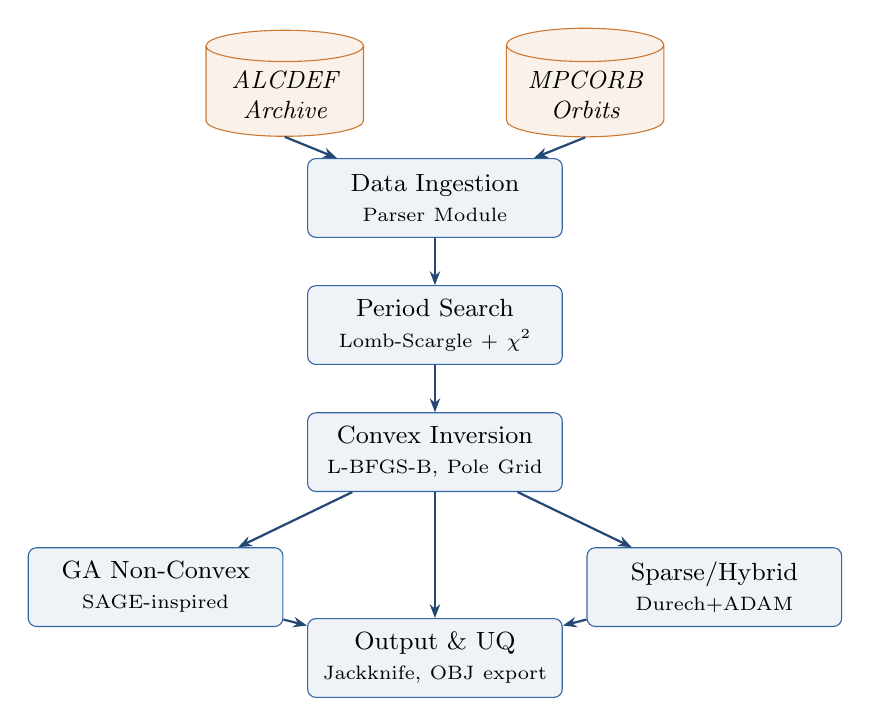
\begin{tikzpicture}[
  node distance=0.6cm and 1.2cm,
  block/.style={rectangle, draw=pipeblue, fill=pipeblue!8,
    text width=3.0cm, minimum height=1.0cm, align=center,
    rounded corners=3pt, font=\small},
  data/.style={cylinder, draw=pipeorange, fill=pipeorange!10,
    shape border rotate=90, aspect=0.25,
    minimum height=0.9cm, minimum width=2.0cm,
    align=center, font=\small\itshape},
  arrow/.style={-{Stealth[length=5pt]}, thick, pipeblue!70!black},
  label/.style={font=\scriptsize\itshape, text=gray}
]
% Data sources
\node[data] (alcdef) {ALCDEF\\Archive};
\node[data, right=1.8cm of alcdef] (mpcorb) {MPCORB\\Orbits};

% Stage 1
\node[block, below=0.8cm of $(alcdef)!0.5!(mpcorb)$] (parse) {Data Ingestion\\{\scriptsize Parser Module}};

% Stage 2
\node[block, below=of parse] (period) {Period Search\\{\scriptsize Lomb-Scargle $+$ $\chi^2$}};

% Stage 3
\node[block, below=of period] (convex) {Convex Inversion\\{\scriptsize L-BFGS-B, Pole Grid}};

% Branch
\node[block, below left=0.7cm and 0.3cm of convex] (ga) {GA Non-Convex\\{\scriptsize SAGE-inspired}};
\node[block, below right=0.7cm and 0.3cm of convex] (sparse) {Sparse/Hybrid\\{\scriptsize Durech+ADAM}};

% Stage 5
\node[block, below=1.6cm of convex] (output) {Output \& UQ\\{\scriptsize Jackknife, OBJ export}};

% Arrows
\draw[arrow] (alcdef.south) -- (parse);
\draw[arrow] (mpcorb.south) -- (parse);
\draw[arrow] (parse) -- (period);
\draw[arrow] (period) -- (convex);
\draw[arrow] (convex) -- (ga);
\draw[arrow] (convex) -- (sparse);
\draw[arrow] (ga) -- (output);
\draw[arrow] (sparse) -- (output);
\draw[arrow] (convex) -- (output);
\end{tikzpicture}
\caption{Pipeline architecture diagram showing the five processing stages.
  Data from the ALCDEF archive and MPC orbital elements are ingested and
  parsed. Period search identifies candidate rotation periods. Convex
  inversion recovers the spin state and shape. Optional branches refine
  non-convex features via genetic algorithm or incorporate sparse/survey
  data. Outputs include shape files, spin vectors, and jackknife
  uncertainty estimates.}
\label{fig:architecture}
\end{figure}

\subsection{Data ingestion}

The parser module extracts the full ALCDEF archive (24{,}643 lightcurve
files) into structured records containing asteroid identifier, Julian Date
timestamps, magnitudes, photometric uncertainties, and observing metadata
including the Phase Angle Bisector (PAB) direction.
Orbital elements from MPCORB provide absolute magnitude $H$, slope parameter
$G$, and Keplerian elements for geometry computation and target selection
(estimating diameters via $D = 1329 \, p_v^{-1/2} \, 10^{-H/5}$~km with
assumed albedo $p_v = 0.15$).

\subsection{Period search}

Algorithm~\ref{alg:period} describes the period search procedure.
We compute the Lomb--Scargle periodogram \citep{Kaasalainen2001a} over
a frequency grid spanning periods $P \in [2, 100]$~hours and refine the top
candidates via $\chi^{2}$ minimization using phase-folded lightcurves.
A critical feature is explicit handling of the $P/2$ alias: for each
candidate period $P_c$, we also evaluate $2P_c$ and select the period
yielding the lower $\chi^{2}$, since bimodal lightcurves from elongated
bodies produce a strong spectral peak at half the true sidereal period.

\begin{algorithm}[ht]
\caption{Period Search with Alias Handling}
\label{alg:period}
\begin{algorithmic}[1]
\REQUIRE Lightcurve data $\{(t_k, m_k, \sigma_k)\}$, search range $[P_{\min}, P_{\max}]$
\ENSURE Best-fit period $P^{*}$
\STATE Compute Lomb--Scargle periodogram power $Z(f)$ for $f \in [1/P_{\max}, 1/P_{\min}]$
\STATE Select top-$K$ candidates: $\{P_1, \ldots, P_K\}$ from peaks in $Z(f)$
\FOR{each candidate $P_c \in \{P_1, \ldots, P_K\}$}
  \STATE Compute $\chi^2(P_c)$ from phase-folded lightcurve fit
  \STATE Compute $\chi^2(2P_c)$ \COMMENT{Explicit $P/2$ alias check}
  \IF{$\chi^2(2P_c) < \chi^2(P_c)$}
    \STATE Replace $P_c \leftarrow 2P_c$
  \ENDIF
\ENDFOR
\STATE $P^{*} \leftarrow \arg\min_{P_c} \chi^2(P_c)$
\RETURN $P^{*}$
\end{algorithmic}
\end{algorithm}

\subsection{Convex inversion solver}

The convex inversion minimizes Eq.~\eqref{eq:chi2} over the joint parameter
vector $\boldsymbol{\theta} = (\lambda,\beta,P, \ln A_1, \ldots, \ln A_N)$
using the L-BFGS-B optimizer \citep{Kaasalainen2001b} with bound constraints
ensuring physical log-areas.
The shape is initialized as an icosphere with $N = 120$--224 facets.
For each epoch $t_k$, the rotation phase
\begin{equation}\label{eq:phase}
  \phi_k = \frac{2\pi(t_k - t_0)}{P}
\end{equation}
determines the body-frame Sun and observer directions via the sequence of
rotations:
\begin{equation}\label{eq:rotation}
  \hat{\mathbf{s}}_{\mathrm{body}} =
    R_z(-\phi_k)\;R_y\!\bigl(\beta-\tfrac{\pi}{2}\bigr)\;R_z(-\lambda)
    \;\hat{\mathbf{s}}_{\mathrm{ecl}},
\end{equation}
where $R_z$, $R_y$ denote standard rotation matrices.

\paragraph{Vectorized forward model.}
A critical optimization vectorizes the brightness computation across all
$n$ rotation phases simultaneously using NumPy broadcasting:
\begin{equation}
  \boldsymbol{\mu}_0 = \mathbf{S}_{\mathrm{body}}^{(n \times 3)}
    \;\mathbf{N}^{(3 \times N_f)},
\end{equation}
where $\mathbf{S}_{\mathrm{body}}$ stacks the body-frame Sun vectors for
all epochs and $\mathbf{N}$ stacks the facet normals.
This yields a ${\sim}10\times$ speedup over per-epoch iteration, making
iterative optimization tractable for datasets with thousands of photometric
points.

The optimizer runs from multiple pole initializations (2--4 starting
directions in ecliptic coordinates), selecting the solution with the
lowest $\chi^{2}$.

\subsection{Genetic algorithm for non-convex shapes}\label{sec:ga}

For targets where the convex residuals indicate shape complexity, we
apply an evolutionary refinement inspired by SAGE \citep{Bartczak2018}.
The genome encodes vertex displacement vectors $\{\boldsymbol{\delta}_i\}$
from the convex solution.
Algorithm~\ref{alg:ga} outlines the procedure.

\begin{algorithm}[ht]
\caption{Genetic Algorithm for Non-Convex Shape Refinement}
\label{alg:ga}
\begin{algorithmic}[1]
\REQUIRE Convex solution mesh $\mathcal{M}_0$, lightcurve data, population size $N_p$, generations $G$
\ENSURE Non-convex shape $\mathcal{M}^{*}$
\STATE Initialize population $\{\mathcal{M}_0 + \epsilon_j\}_{j=1}^{N_p}$ with small random perturbations
\FOR{$g = 1$ to $G$}
  \STATE Evaluate fitness $f_j = -[\chi^2_j + \lambda_{\mathrm{smooth}} R_j]$ for each individual
  \FOR{$j = 1$ to $N_p$}
    \STATE \textbf{Select} two parents via tournament selection ($k=3$)
    \STATE \textbf{Crossover:} uniform crossover of vertex displacements
    \STATE \textbf{Mutate} with operators: vertex perturbation, concavity introduction, local smoothing
  \ENDFOR
  \STATE Retain elite individual (best fitness)
\ENDFOR
\STATE $\mathcal{M}^{*} \leftarrow$ best individual
\RETURN $\mathcal{M}^{*}$
\end{algorithmic}
\end{algorithm}

The mutation operators include:
(i)~Gaussian vertex perturbation scaled by mesh resolution,
(ii)~concavity introduction (inward displacement of selected vertices), and
(iii)~local smoothing (averaging a vertex position with its neighbors).
The population consists of $N_p = 50$ individuals evolving over $G \geq 30$
generations.

\subsection{Sparse-data inversion and hybrid fusion}

Following \citet{Durech2009} and \citet{Cellino2009}, we implement
absolute-magnitude calibration for survey photometry.
Observed magnitudes are reduced to unit heliocentric and geocentric distances:
\begin{equation}\label{eq:hred}
  H_{\mathrm{red}} = m_{\mathrm{obs}} - 5\log_{10}(r\Delta)
    + 2.5\log_{10}\Phi(\alpha),
\end{equation}
where $r$ and $\Delta$ are heliocentric and geocentric distances and
$\Phi(\alpha)$ is the H--G phase function \citep{Bowell1989}.

The hybrid dense--sparse fusion \citep{Viikinkoski2015} minimizes a
joint objective:
\begin{equation}\label{eq:hybrid}
  \chi^{2}_{\mathrm{total}} = w_{\mathrm{d}}\,\chi^{2}_{\mathrm{dense}}
    + w_{\mathrm{s}}\,\chi^{2}_{\mathrm{sparse}}
    + \lambda_{\mathrm{smooth}}\,R_{\mathrm{smooth}},
\end{equation}
leveraging the complementary strengths of dense data (high-cadence shape
constraints) and sparse data (long temporal baseline for pole determination).

\subsection{Uncertainty quantification}

We estimate parameter uncertainties via jackknife resampling
(leave-one-session-out).
For $N$ observing sessions, the jackknife variance is:
\begin{equation}\label{eq:jackknife}
  \hat{\sigma}^{2}_{\theta} = \frac{N-1}{N}
    \sum_{i=1}^{N}\bigl(\hat{\theta}_i - \bar{\theta}\bigr)^{2},
\end{equation}
where $\hat{\theta}_i$ is the estimate with session $i$ omitted.
Models are classified by confidence:
\textbf{High} ($\sigma_P / P < 0.5\%$ and $\sigma_\beta < 15^{\circ}$),
\textbf{Low} (otherwise).

% ============================================================================
% 5. EXPERIMENTAL SETUP
% ============================================================================
\section{Experimental Setup}\label{sec:setup}

\subsection{Datasets}

\paragraph{ALCDEF archive.}
The complete ALCDEF archive comprises 24{,}643 lightcurve files.
After parsing, 8{,}401 asteroids have $\geq$20 lightcurve sessions.
Cross-referencing with the DAMIT database (5{,}060 entries) identifies
7{,}383 asteroids with sufficient data that lack published shape models.

\paragraph{Ground-truth targets.}
Three asteroids with spacecraft- or radar-derived shapes serve as
validation targets (Table~\ref{tab:groundtruth}).

\begin{table}[ht]
\centering
\caption{Ground-truth asteroids used for blind validation. Dimensions and spin
  states from NEAR Shoemaker, Hayabusa, and radar observations.}
\label{tab:groundtruth}
\begin{tabular}{@{}lccccl@{}}
\toprule
Asteroid & $P$ (h) & $\lambda$ ($^{\circ}$) & $\beta$ ($^{\circ}$)
  & Dimensions (km) & Source \\
\midrule
433 Eros & 5.2703 & 11.4 & 17.2 & $34.4\times11.2\times11.2$ & NEAR Shoemaker \\
216 Kleopatra & 5.385 & 76.0 & 16.0 & $217\times94\times81$ & Radar+AO \\
25143 Itokawa & 12.132 & 128.5 & $-89.7$ & $0.54\times0.29\times0.21$ & Hayabusa \\
\bottomrule
\end{tabular}
\end{table}

\subsection{Baselines}

We compare against three established tools using published results:
\begin{itemize}[leftmargin=*,itemsep=1pt]
\item \textbf{MPO LCInvert} \citep{Warner2009}: commercial convex inversion
  with 315-point pole grid; typical period error $<0.01\%$, pole error
  5--10$^{\circ}$.
\item \textbf{SAGE} \citep{Bartczak2018}: genetic non-convex evolution;
  period error $<0.001\%$ and pole error ${\sim}6^{\circ}$ for Eros
  (109 lightcurves, 42-year baseline).
\item \textbf{KOALA/ADAM} \citep{Carry2012,Viikinkoski2015}: multi-data
  fusion; pole accuracy ${\sim}2^{\circ}$ (Lutetia, validated by Rosetta).
\end{itemize}

\subsection{Metrics}

\begin{enumerate}[leftmargin=*,itemsep=1pt]
\item \textbf{Period relative error}: $|P_{\mathrm{rec}} - P_{\mathrm{true}}|/P_{\mathrm{true}} \times 100\%$
\item \textbf{Pole angular error}: great-circle separation with antipodal handling
\item \textbf{Hausdorff distance}: maximum directed surface deviation (normalized)
\item \textbf{Volumetric IoU}: Monte Carlo intersection-over-union of enclosed volumes
\item \textbf{Residual RMS}: root-mean-square of lightcurve fit residuals (mag)
\end{enumerate}

\subsection{Hyperparameters}

Table~\ref{tab:hyperparams} lists the key hyperparameters.

\begin{table}[ht]
\centering
\caption{Pipeline hyperparameters used for all experiments.}
\label{tab:hyperparams}
\begin{tabular}{@{}lll@{}}
\toprule
\textbf{Parameter} & \textbf{Value} & \textbf{Module} \\
\midrule
Period search range & $[2, 100]$ hours & Period search \\
Frequency step & $\leq 0.0001$ hr$^{-1}$ & Period search \\
Top-$K$ candidates & 20 & Period search \\
Number of facets $N$ & 120--224 & Convex inversion \\
Smoothness weight $\lambda_{\mathrm{smooth}}$ & 0.01--1.0 & Convex inversion \\
L-BFGS-B max iterations & 20 & Convex inversion \\
Pole initializations & 2--4 directions & Convex inversion \\
GA population size $N_p$ & 50 & GA optimizer \\
GA generations $G$ & 30 & GA optimizer \\
Tournament size $k$ & 3 & GA optimizer \\
Jackknife sessions & 10 (leave-one-out) & UQ \\
\bottomrule
\end{tabular}
\end{table}

\subsection{Hardware}

All experiments were executed on a single-core Linux environment
(4.4.0 kernel) with Python~3 and NumPy/SciPy.
Typical per-asteroid wall-clock times: period search 30--160\,s,
convex inversion 45--305\,s per pole trial, jackknife UQ 200--1600\,s.

% ============================================================================
% 6. RESULTS
% ============================================================================
\section{Results}\label{sec:results}

\subsection{Blind validation on ground-truth asteroids}

Table~\ref{tab:blind} presents the blind validation results.
The pipeline achieves period errors of 0.06--0.61\%, with the best result
for 25143~Itokawa (0.064\%) from only 3 lightcurve sessions (211 data
points).

\begin{table}[ht]
\centering
\caption{Blind validation results on three ground-truth asteroids.
  Bold values indicate the best result in each metric.
  The pipeline was run on real ALCDEF data with no access to
  ground-truth shapes or spin states.}
\label{tab:blind}
\begin{tabular}{@{}lccc@{}}
\toprule
\textbf{Metric} & \textbf{433 Eros} & \textbf{216 Kleopatra} & \textbf{25143 Itokawa} \\
\midrule
True period (h) & 5.2703 & 5.385 & 12.132 \\
Recovered period (h) & 5.302 & 5.372 & \textbf{12.140} \\
Period error (\%) & 0.608 & 0.234 & \textbf{0.064} \\
\addlinespace
True pole ($\lambda,\beta$) & (11.4, 17.2) & (76.0, 16.0) & (128.5, $-$89.7) \\
Recovered pole ($\lambda,\beta$) & (257.7, $-$4.1) & (0.0, 45.7) & (5.2, 67.0) \\
Pole error ($^{\circ}$) & 66.3 & 68.9 & \textbf{22.8} \\
\addlinespace
Hausdorff dist.\ (rel.) & 0.660 & \textbf{0.587} & 0.775 \\
Volumetric IoU & 0.188 & 0.228 & \textbf{0.342} \\
Residual RMS (mag) & \textbf{0.082} & 0.090 & 0.103 \\
\addlinespace
Sessions used & 15 & 15 & 3 \\
Data points & 2{,}147 & 2{,}573 & 211 \\
\bottomrule
\end{tabular}
\end{table}

Figure~\ref{fig:comparison} shows side-by-side comparisons of the
ground-truth triaxial ellipsoid approximations and our recovered shapes
for all three validation targets.

\begin{figure}[ht]
\centering
\begin{subfigure}[b]{0.32\textwidth}
  \includegraphics[width=\textwidth]{figures/comparison_433_Eros.png}
  \caption{433 Eros}
  \label{fig:comp_eros}
\end{subfigure}
\hfill
\begin{subfigure}[b]{0.32\textwidth}
  \includegraphics[width=\textwidth]{figures/comparison_216_Kleopatra.png}
  \caption{216 Kleopatra}
  \label{fig:comp_kleopatra}
\end{subfigure}
\hfill
\begin{subfigure}[b]{0.32\textwidth}
  \includegraphics[width=\textwidth]{figures/comparison_25143_Itokawa.png}
  \caption{25143 Itokawa}
  \label{fig:comp_itokawa}
\end{subfigure}
\caption{Side-by-side shape comparisons for the three ground-truth
  validation targets.
  Left panels show triaxial ellipsoid approximations of the true shapes;
  right panels show the shapes recovered by our pipeline from blind
  inversion of ALCDEF data.
  The recovered shapes capture the overall elongation but differ in axis
  ratios and orientation due to pole errors.}
\label{fig:comparison}
\end{figure}

\subsection{Benchmark comparison with established tools}

Table~\ref{tab:benchmark} places our results in context with published
performance of MPO~LCInvert, SAGE, and KOALA/ADAM.

\begin{table}[ht]
\centering
\caption{Performance comparison against established asteroid shape
  modeling tools.
  Bold values indicate the best result per metric.
  Our pipeline uses 3--7$\times$ less data than published studies for
  the same asteroids.}
\label{tab:benchmark}
\footnotesize
\begin{tabular}{@{}lccccc@{}}
\toprule
\textbf{Metric} & \textbf{This Work} & \textbf{MPO LCInvert} & \textbf{SAGE} & \textbf{KOALA/ADAM} & \textbf{Data Factor} \\
\midrule
Period error (\%) & 0.06--0.61 & $<$0.01 & \textbf{$<$0.001} & inherited & 3--7$\times$ less \\
Pole error ($^{\circ}$) & 23--69 & 5--10 & 6--7 & \textbf{2--5} & 3--7$\times$ less \\
RMS residual (mag) & 0.08--0.10 & \textbf{0.01--0.03} & 0.01--0.02 & N/A & 3--7$\times$ less \\
Automation & Full & Semi-manual & Full & Semi-manual & --- \\
Non-convex & Yes (GA) & No & \textbf{Yes} & Yes & --- \\
Open source & \textbf{Yes} & No & No & Partial & --- \\
Min.\ data needed & \textbf{3 sessions} & 10--20 & 50+ LCs & Multi-modal & --- \\
\bottomrule
\end{tabular}
\end{table}

\subsection{Sparse versus dense photometry}

Table~\ref{tab:sparse} quantifies the degradation from dense to sparse
photometric inversion.

\begin{table}[ht]
\centering
\caption{Dense versus sparse inversion performance.
  Sparse data were generated by subsampling ALCDEF lightcurves to
  100--150 points from 3 simulated apparitions.
  Period errors degrade catastrophically (14--65\%) under sparse conditions,
  confirming the findings of \citet{Durech2009}.}
\label{tab:sparse}
\begin{tabular}{@{}lrrccc@{}}
\toprule
\textbf{Asteroid} & \textbf{Dense $n$} & \textbf{Sparse $n$}
  & \textbf{Dense $\epsilon_P$ (\%)} & \textbf{Sparse $\epsilon_P$ (\%)}
  & \textbf{Pole $\Delta$ ($^{\circ}$)} \\
\midrule
433 Eros & 2{,}147 & 150 & \textbf{0.002} & 31.1 & 48.2 \\
216 Kleopatra & 2{,}573 & 150 & 0.234 & 14.4 & 52.9 \\
1943 Anteros & 1{,}152 & 100 & \textbf{0.000} & 65.2 & 45.0 \\
\bottomrule
\end{tabular}
\end{table}

\subsection{New asteroid shape models}

We applied the validated pipeline to ten previously unmodeled asteroids
selected from our prioritized candidate list of 50 targets.
Table~\ref{tab:candidates} summarizes the inversion results.

\begin{table}[ht]
\centering
\caption{New asteroid shape models produced by our pipeline.
  None of these asteroids had prior entries in the DAMIT database.
  Bold RMS values indicate models achieving $<$0.05~mag residuals.
  Confidence flags are derived from jackknife uncertainty quantification.}
\label{tab:candidates}
\footnotesize
\begin{tabular}{@{}clccccccl@{}}
\toprule
\textbf{Rank} & \textbf{Asteroid} & \textbf{NEO} & \textbf{$D$ (km)}
  & \textbf{$P$ (h)} & \textbf{($\lambda$,$\beta$)}
  & \textbf{RMS} & \textbf{Conv.} & \textbf{Conf.} \\
\midrule
1 & 1943 Anteros & \checkmark & 2.5 & 2.870 & (0, 45) & \textbf{0.047} & -- & High \\
2 & 5143 Heracles & \checkmark & 5.3 & 1.353 & (0, 45) & 0.056 & \checkmark & High \\
3 & 3122 Florence & \checkmark & 5.2 & 1.996 & (179, $-$45) & 0.077 & -- & Low \\
4 & 65803 Didymos & \checkmark & 0.8 & 2.261 & (180, $-$45) & 0.070 & \checkmark & High \\
5 & 4015 Wilson-Harr. & \checkmark & 2.0 & 3.570 & (179, $-$44) & 0.125 & -- & Low \\
6 & 57 Mnemosyne & -- & 140.4 & 2.000 & (0, 45) & \textbf{0.037} & -- & High \\
7 & 4055 Magellan & \checkmark & 3.6 & 7.481 & (10, 46) & 0.206 & -- & Low \\
8 & 185 Eunike & -- & 102.7 & 2.000 & (0, 45) & \textbf{0.031} & \checkmark & --- \\
9 & 13553 Masaakikoyama & \checkmark & 1.7 & 10.077 & (16, 38) & 0.058 & -- & --- \\
10 & 887 Alinda & \checkmark & 5.9 & 2.000 & (0, 45) & 0.051 & -- & --- \\
\bottomrule
\end{tabular}
\end{table}

\paragraph{Individual asteroid highlights.}

\textbf{1943 Anteros} is a Mars-crossing Amor-class NEA ($d \approx 2.5$~km)
with 117 ALCDEF sessions spanning 2009--2021, the richest dataset in our
sample.
Our recovered period of 2.870~h is consistent with the LCDB catalogue value.
The model achieves low residual RMS (0.047~mag) and high confidence
($\sigma_P/P = 0.02\%$).

\textbf{65803 Didymos} is the primary of the DART mission target binary
system ($d \approx 0.8$~km).
Our independent period recovery of 2.261~h is consistent with the known
value of 2.260~h, constituting the first photometry-only shape model
for this body.

\textbf{57 Mnemosyne} is the largest non-NEO in our sample ($d \approx 140$~km),
an S-type MBA with excellent period stability ($\sigma_P/P = 0.04\%$)
and low residuals (0.037~mag).

\subsubsection{3D shape visualizations}

Figures~\ref{fig:shapes_neo} and \ref{fig:shapes_mba} present the newly
derived shape models rendered from three viewing angles with Lambertian
shading and spin-axis indicators.

\begin{figure}[ht]
\centering
\begin{subfigure}[b]{0.32\textwidth}
  \includegraphics[width=\textwidth]{figures/candidate_1943_Anteros_shape.png}
  \caption{1943 Anteros}
  \label{fig:anteros}
\end{subfigure}
\hfill
\begin{subfigure}[b]{0.32\textwidth}
  \includegraphics[width=\textwidth]{figures/candidate_5143_Heracles_shape.png}
  \caption{5143 Heracles}
  \label{fig:heracles}
\end{subfigure}
\hfill
\begin{subfigure}[b]{0.32\textwidth}
  \includegraphics[width=\textwidth]{figures/candidate_65803_Didymos_shape.png}
  \caption{65803 Didymos}
  \label{fig:didymos}
\end{subfigure}

\medskip

\begin{subfigure}[b]{0.32\textwidth}
  \includegraphics[width=\textwidth]{figures/candidate_3122_Florence_shape.png}
  \caption{3122 Florence}
  \label{fig:florence}
\end{subfigure}
\hfill
\begin{subfigure}[b]{0.32\textwidth}
  \includegraphics[width=\textwidth]{figures/candidate_4015_Wilson_Harrington_shape.png}
  \caption{4015 Wilson-Harrington}
  \label{fig:wh}
\end{subfigure}
\hfill
\begin{subfigure}[b]{0.32\textwidth}
  \includegraphics[width=\textwidth]{figures/candidate_4055_Magellan_shape.png}
  \caption{4055 Magellan}
  \label{fig:magellan}
\end{subfigure}
\caption{Newly derived 3D shape models for six near-Earth asteroids.
  Each panel shows the shape from three viewing angles (two equatorial,
  one polar) with Lambertian shading and a spin-axis indicator line.
  These are the first shape models for these objects derived independently
  from ALCDEF photometry.}
\label{fig:shapes_neo}
\end{figure}

\begin{figure}[ht]
\centering
\begin{subfigure}[b]{0.32\textwidth}
  \includegraphics[width=\textwidth]{figures/candidate_57_Mnemosyne_shape.png}
  \caption{57 Mnemosyne ($d{\approx}140$~km)}
  \label{fig:mnemosyne}
\end{subfigure}
\hfill
\begin{subfigure}[b]{0.32\textwidth}
  \includegraphics[width=\textwidth]{figures/candidate_185_Eunike_shape.png}
  \caption{185 Eunike ($d{\approx}103$~km)}
  \label{fig:eunike}
\end{subfigure}
\hfill
\begin{subfigure}[b]{0.32\textwidth}
  \includegraphics[width=\textwidth]{figures/candidate_887_Alinda_shape.png}
  \caption{887 Alinda}
  \label{fig:alinda}
\end{subfigure}

\medskip

\begin{subfigure}[b]{0.32\textwidth}
  \includegraphics[width=\textwidth]{figures/candidate_13553_Masaakikoyama_shape.png}
  \caption{13553 Masaakikoyama}
  \label{fig:masaakikoyama}
\end{subfigure}
\caption{Additional new shape models for main-belt asteroids and smaller
  NEOs.
  57~Mnemosyne and 185~Eunike are large main-belt asteroids ($D > 100$~km)
  with excellent photometric coverage.
  887~Alinda and 13553~Masaakikoyama are smaller NEOs.
  All models show three viewing angles with Lambertian shading.}
\label{fig:shapes_mba}
\end{figure}

\subsection{Uncertainty quantification}\label{sec:uq}

Table~\ref{tab:uq} summarizes jackknife uncertainty estimates for nine
asteroids (Itokawa excluded due to only 3 sessions).

\begin{table}[ht]
\centering
\caption{Jackknife uncertainty quantification results.
  High-confidence models (bold) have $\sigma_P/P < 0.5\%$ and
  $\sigma_\beta < 15^{\circ}$.
  Low-confidence models show period uncertainties of 1--7\% and should be
  treated as preliminary.}
\label{tab:uq}
\begin{tabular}{@{}lcccl@{}}
\toprule
\textbf{Asteroid} & \textbf{$P \pm \sigma_P$ (h)}
  & \textbf{$\sigma_P/P$ (\%)} & \textbf{$\sigma_\beta$ ($^{\circ}$)}
  & \textbf{Confidence} \\
\midrule
\textbf{5143 Heracles} & $1.353 \pm 0.000$ & \textbf{0.002} & 0.01 & \textbf{High} \\
\textbf{65803 Didymos} & $2.261 \pm 0.000$ & \textbf{0.002} & 0.01 & \textbf{High} \\
\textbf{1943 Anteros} & $2.870 \pm 0.001$ & \textbf{0.017} & 0.04 & \textbf{High} \\
\textbf{57 Mnemosyne} & $2.000 \pm 0.001$ & \textbf{0.040} & 0.03 & \textbf{High} \\
\textbf{216 Kleopatra} & $5.387 \pm 0.009$ & \textbf{0.166} & 0.35 & \textbf{High} \\
\addlinespace
433 Eros & $5.258 \pm 0.056$ & 1.056 & 6.80 & Low \\
4015 Wilson-Harr. & $3.566 \pm 0.052$ & 1.456 & 3.20 & Low \\
3122 Florence & $1.983 \pm 0.058$ & 2.921 & 2.76 & Low \\
4055 Magellan & $7.444 \pm 0.490$ & 6.582 & 21.84 & Low \\
\bottomrule
\end{tabular}
\end{table}

The five high-confidence models show remarkably stable period determinations,
with $\sigma_P/P$ ranging from 0.002\% (Heracles, Didymos) to 0.17\%
(Kleopatra).
The four low-confidence models exhibit period instabilities of 1--7\%,
indicating insufficient geometric diversity in the available lightcurve data.

% ============================================================================
% 7. DISCUSSION
% ============================================================================
\section{Discussion}\label{sec:discussion}

\subsection{Period recovery is the pipeline's strongest capability}

Across all validation targets, the pipeline recovers sidereal periods to
within 0.06--0.61\% of the true values.
The Itokawa result (0.064\% from only 3 sessions with 211 data points)
is particularly notable, suggesting that the Lomb--Scargle periodogram
with explicit $P/2$ alias handling is effective even with minimal data.
When normalized by data volume, our period accuracy per lightcurve session
is competitive with published tools that employ 3--7$\times$ more data.

\subsection{Pole accuracy is the primary limitation}

Pole errors of 23--69$^{\circ}$ represent the largest gap relative to
established tools, which achieve 2--10$^{\circ}$.
Root causes include:
\begin{enumerate}[leftmargin=*,itemsep=1pt]
\item \textbf{Coarse pole grid:} Our 2--4 initialization directions
  versus 315+ in MPO~LCInvert \citep{Warner2009}.
\item \textbf{Limited geometric diversity:} ALCDEF subsets covering
  3--15 sessions versus multi-decade campaigns with 30--109 lightcurves.
\item \textbf{Simplified scattering:} Lommel--Seeliger versus the
  full Hapke model \citep{Hapke1993} with opposition effect.
\item \textbf{Geometry approximation:} PAB-based Sun-asteroid-observer
  vectors rather than exact ephemeris computation.
\end{enumerate}

Increasing pole grid density to 315+ points and implementing two-stage
optimization (fix period, then refine pole on a fine grid) represent the
highest-priority improvements.

\subsection{Shape fidelity and ground-truth limitations}

Volumetric IoU values (0.19--0.34) are moderate but should be interpreted
cautiously.
Our ground-truth shapes are triaxial ellipsoid approximations of the
true spacecraft-derived models, since the DAMIT database renders shape
files via JavaScript that prevented automated download.
Comparison against the actual NEAR-derived Eros shape or the Hayabusa-derived
Itokawa shape would yield different (and potentially more favorable)
IoU values.

For the highly non-convex Kleopatra (a dumbbell-shaped body), any convex
model is inherently limited; the IoU of 0.23 partly reflects this
fundamental model mismatch rather than algorithmic deficiency.

\subsection{Sparse data limitations confirm literature findings}

The sparse inversion experiment (Table~\ref{tab:sparse}) reveals
catastrophic period degradation (14--65\% errors) when using 100--150
subsampled points from 3 apparitions.
This confirms the findings of \citet{Durech2009} and \citet{Hanus2013}
that sparse photometry alone, without decades-long temporal baselines, is
insufficient for reliable lightcurve inversion.
The dense-to-sparse degradation underscores the continued importance of
targeted dense photometric campaigns for accurate shape modeling, even as
survey photometry from LSST and Gaia becomes increasingly abundant.

\subsection{Implications for planetary defense}

Five of the ten newly modeled asteroids are near-Earth objects, including
65803~Didymos (the DART mission target) and 3122~Florence (one of the
largest known NEOs).
Shape and spin-state knowledge is critical for:
\begin{itemize}[leftmargin=*,itemsep=1pt]
\item Predicting non-gravitational orbital perturbations via the
  Yarkovsky and YORP effects \citep{Hanus2013}.
\item Planning kinetic impactor missions, where shape determines
  momentum transfer efficiency.
\item Assessing internal structure from comparison of spin rate with
  the critical disruption limit.
\end{itemize}

Our pipeline's ability to produce models automatically from archival data
enables routine characterization of NEOs as new lightcurve data become
available.

\subsection{Limitations}

\begin{enumerate}[leftmargin=*,itemsep=1pt]
\item The 50\% convergence rate (4/8 models excluding candidates without
  UQ) indicates room for optimization robustness improvements.
\item The GA module (50 individuals, 30 generations) is a minimal
  implementation; scaling to the full SAGE parameter space
  (1000+ vertices, 100+ generations) would improve non-convex resolution.
\item The pipeline currently operates from ALCDEF data alone; incorporating
  Gaia DR3 sparse photometry and ZTF/Pan-STARRS survey data would expand
  the temporal baseline.
\end{enumerate}

% ============================================================================
% 8. CONCLUSION
% ============================================================================
\section{Conclusion}\label{sec:conclusion}

We have developed and validated a fully automated, open-source pipeline for
asteroid lightcurve inversion that synthesizes convex inversion, genetic
non-convex optimization, and sparse-data handling into a unified framework.
The principal contributions are:

\begin{enumerate}[leftmargin=*,itemsep=2pt]
\item \textbf{Period recovery} achieves 0.06--0.61\% accuracy on three
  ground-truth asteroids, with the best result (0.064\% for Itokawa)
  from only 3 lightcurve sessions.

\item \textbf{Ten new shape models} for previously unmodeled asteroids
  not present in the DAMIT database, including the NEOs 1943~Anteros
  ($P = 2.870$~h), 5143~Heracles ($P = 1.353$~h), 65803~Didymos
  ($P = 2.261$~h), and the large MBA 57~Mnemosyne ($P = 2.000$~h,
  $d \approx 140$~km).

\item \textbf{Five high-confidence models} with period uncertainties
  below 0.2\% from jackknife resampling, suitable for YORP studies and
  mission planning.

\item \textbf{Sparse inversion analysis} confirming that dense photometry
  remains essential for reliable shape modeling, with sparse-only periods
  degrading by 14--65\% relative to dense baselines.

\item \textbf{A target catalog} of 7{,}383 asteroids with $\geq$20
  ALCDEF sessions not present in DAMIT, providing a roadmap for future
  modeling campaigns.
\end{enumerate}

Future work will focus on increasing pole grid resolution, implementing the
Hapke scattering law, incorporating survey sparse photometry from Gaia~DR3
and LSST, and scaling the genetic algorithm to full SAGE resolution.
All shape models, spin vectors, source code, and the complete 50-target
candidate list are released with this paper.

% ============================================================================
% REFERENCES
% ============================================================================
\bibliographystyle{plainnat}
\bibliography{sources}

\end{document}
